\section{Implementation}

\subsection{Architecture}

\subsubsection{Data Structures and Overview}
For conveniently accessing the data contained in the wave file, we created the WaveFileWrapper class. The wrapper is used by the home components to access the relevant data needed to create a frame collection. 

\begin{figure}[H]
    \centering
    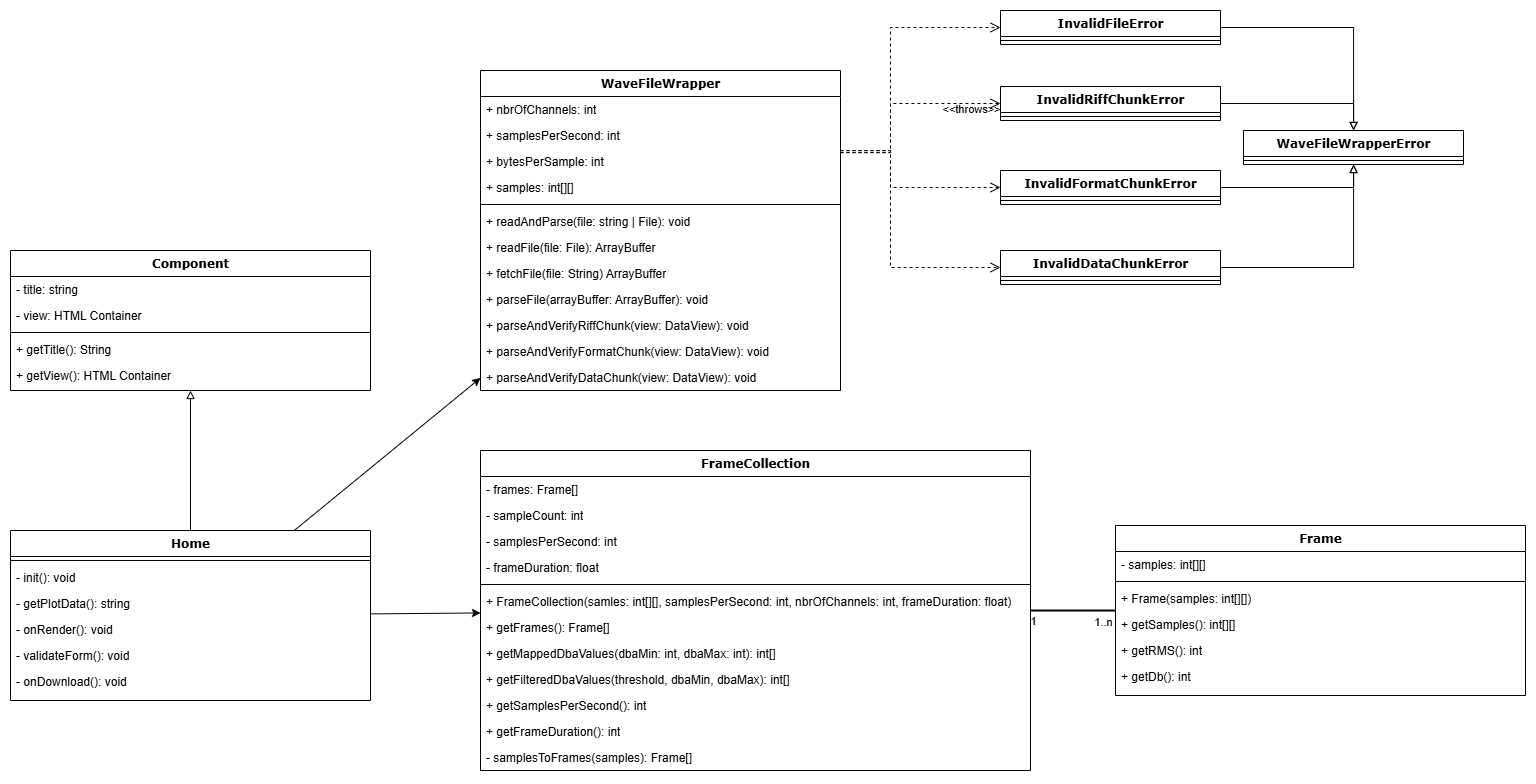
\includegraphics[width=0.8\textwidth]{../assets/class_diagram.png}
    \caption{Class diagram}
\end{figure}

\subsubsection{JavaScript Frontend (SPA)}
The frontend hosted on \href{https://decibel-threshold-event-displayer.github.io/}{Github Pages} is implemented as a single page application (SPA) following the architecture provided by the BFH in the module BTI1301 Web Programming.
In this architecture, the web server provides the index.html file as and uses JavaScript to manage the web contents (DOM updates) without changing the HTML file itself. Currently, the application only has one route; however, the project team chose to
implement a small framework allowing for future expansion without rewriting the entire application. Since the application uses SwiftLaTeX, which is run locally using WebAssembly, the SPA provides an interface for the PDF engine to
its components.
\begin{figure}[H]
    \centering
    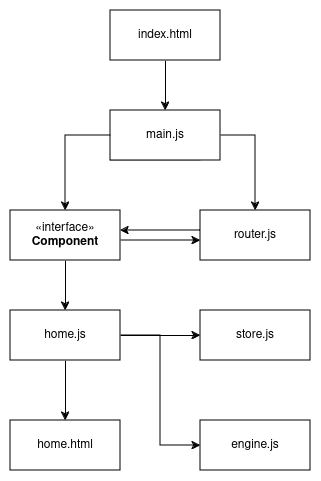
\includegraphics[width=0.4\textwidth]{../assets/spa_diagram.png}
    \caption{SPA Architecture}
\end{figure}
In order to ensure a consistent and agreeable look, the project team has decided to use \href{https://getbootstrap.com/}{Bootstrap}, which is \href{https://github.com/twbs/bootstrap/blob/main/LICENSE}{licensed under MIT}.

\subsubsection{High-Level architecture}
!TODO: we should put this either at the beginning or end of this chapter to show what the entire architecture looks like high-level!

\subsection{Processes}
The following diagram shows which steps are involved when creating a noise report from a wave file.

\begin{figure}[H]
    \centering
    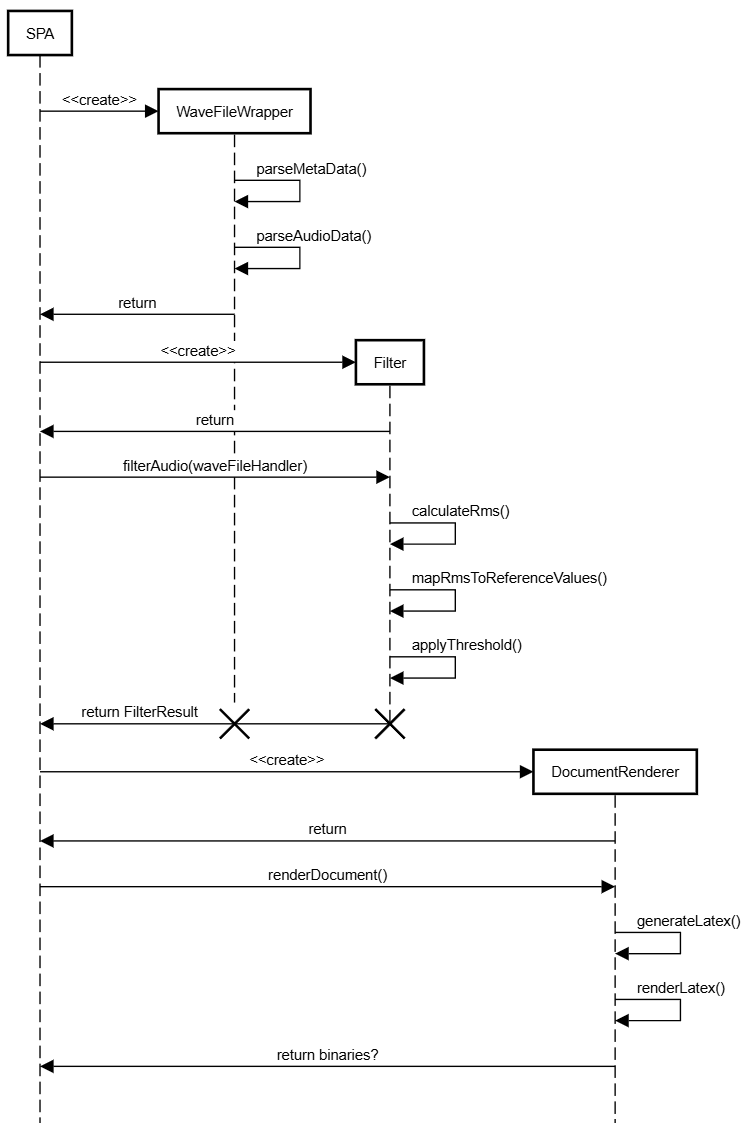
\includegraphics[width=0.8\textwidth]{../assets/sequence_diagram_from_wave_file_to_pdf.png}
    \caption{Sequence diagram of steps involved when creating a noise report}
\end{figure}

\subsubsection{Parsing the Wave File}
The WaveFileWrapper class will be responsible for reading and parsing the wave file. Reading a file in a web context always works asynchronous, which is why there is a helper function "readAndParse" which has to be called with async await.
The format itself is straight forward\cite{wav_file_format_wikipedia}, the only important thing is that the whole file is Little-Endian.
It starts with a 12 byte header which we use to verify that the given file is actually a wave file.
After the header comes a 24 byte chunk which contains information about the data format.
We are interested in the following fields:
\begin{itemize}
    \item AudioFormat (2 bytes): we only support PCM and IEEE Float format
    \item NbrChannels (2 bytes): is used to parse individual samples
    \item Frequence (4 bytes): number of samples per second, this is needed for filtering and summarising
    \item BitsPerSample (2 bytes): number of bits for a single sample for a single channel, is used to parse individual samples
\end{itemize}
After the format chunk comes an optional list chunk containing some additional metadata in which we are not interested.
There we skip that chunk and go straight to the data chunk.
This chunk starts with a 4 byte long DataBlocID, which should always have the value 'data'.
The next 4 byte represent the number of samples in the data.
After that comes the actual audio data.
To parse a single sample, we need to parse a frame.
A frame contains the data of all channels and has therefore a size of \[\frac{NbrChannels * BitsPerSample}{8}\] bytes.

\subsubsection{Calculating Decibel Values}
If an audio file consists of several channels, we use the average of the channels as the value of the sample.
When we want to analyze where a certain decibel threshold has been exceeded, we must have accurate values.
People only perceive something as loud if it is loud over a longer period of time.
Short peaks are perceived less.
Therefore, when determining the effective loudness of audio, we do not use the loudness of individual samples, but rather the average of a number of samples over a certain period of time. We will, as usual when working with audio, use the root mean squere (RMS), as we are interested in the absolute amplitude values.
The calculated average then depends heavily on how long the time period is.
In practice, 300ms is usually used\cite{timespan_for_audio_rms_calculate}.
This is also the default value, which can be adjusted by the user via the settings.
The decibel value is calculated with the following formula\cite{decibel_wikipedia}:
\[20 * \log_{10} (sample)\]

As mentioned in the introduction, the audio file only contains relative values.
We therefore need to map the RMS values to the number range of the reference values, where the smallest sample is mapped to the minimal dB(A) and the largest sample is mapped to the maximal dB(A) measured.

\subsubsection{Performance improvements}
Generating the PDF file from a LaTeX document in the browser takes quite some time, as it loads all dependencies
on the fly.
To speed up this process, we serve all required LaTeX files ourselves and prefetch them in parallel.
This means we have to download all LaTeX files from a public source, we are using the same source as SwiftLaTeX:
\href{https://texlive2.swiftlatex.com/}{texlive2.swiftlatex.com}

We collected all required LaTeX dependencies by modifying the SwiftLaTeX JavaScript, in such a way that during a sample
all requests pdf generation, are stored in an array, which is then printed to the console.
We put the console output in the file ``app/dependencies.json`` and created a python script under ``app/download\_dependencies.py``,
which downloads all LaTeX files to the directory ``app/dependencies/``.
We then copied the contents of ``app/dependencies.json`` to ``app/dependencies.local.json`` and made the paths relative.
Now we load this file in our main JavaScript file ``app/app.js`` and use ``Promise.all`` together with ``fetch`` to load
all dependencies into the cache of the browser.

Currently, this process involves some manual steps and could be automated in a later step.

\subsection{Testing}
Because we don't use any Frontend Framework and instead build our own SPA, we don't have a testing framework to use. We therefore decides to build 
our own rudimentary testing framework. It consists out of 4 assert functions, a test runner and a html page for displaying the results.
There is no automatic mechanism running the tests after every commit, the tests have to be run manually. 

As we are developing an application for analyzing a wave file, nearly every tests first step is to create a WaveFileWrapper object for further use. Because the reading and parsing of the file works asynchronous, the test suit has also to be asynchronous. We decided to use the async/wait approach instead of using promises because promises are more difficult to debug, which is not suitable for a test framework.

\begin{figure}[H]
    \centering
    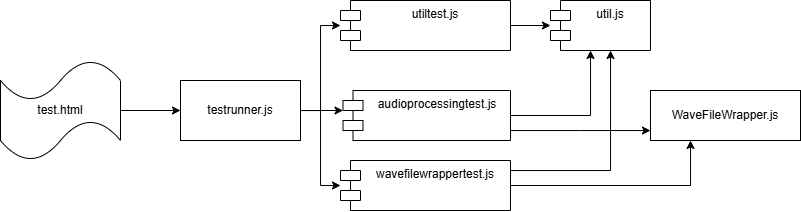
\includegraphics[width=\textwidth]{../assets/overview_test_framework.png}
    \caption{Overview test framework}
\end{figure}

\subsubsection{Assert functions}
For implementing tests there are 5 assert functions contained in the util module which can be used:

\begin{itemize}
    \item assertThrows: verifies that a certain exception is thrown
    \item assertNotThrows: verifies that no exception is thrown
    \item assertEquals: verifies that something is equal to a given value
    \item assertNotEquals: verifies that something is not equal to a given value
    \item assertGreaterThen: verifies that a number is greater the the other
\end{itemize}

If the assertion of a function fails, it throws an exception with some information on why the test failed.
The assertEquals and assertNotEquals function work with any kind of object. They first stringify both objects to a json format and then compare the json. It is certainly not the most efficient method, but it works for all cases. The assertThrows and assertNotThrows both take in a function which will be called in the assert function it self and verified that it throws or not throws an exception. The assertGreaterThen can also take in two arguments from any type, as javascript allows such comparions. With those functions we were able to implement all our tests. 
To make sure that the assert functions work, we implemented also tests for them. Those test obviously don't use the assert functions and rather have some hard coded tests created for them. Those tests can be found in the utiltest module.

\subsubsection{Creating tests}
To create tests, one has to create a javascript file containing its tests. All functions that are beeing exported by the given javascript file are considered to be tests and will be executed by the test runner. If a function throws an expection, it is assumed that the test failed. If no exception is thrown, the test passes. 
We tried to keep the manual work for adding tests minimal, but some manual work is still necessary. To add a new test module, the module has to be imported into the test runner file. After that, a new call to the function runTestGroup can be added, which will then add the test. Thats it.

\begin{figure}[H]
    \centering
    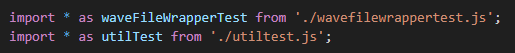
\includegraphics[width=0.8\textwidth]{../assets/import_test_module.png}
    \caption{Importing a module with tests}
\end{figure}

\begin{figure}[H]
    \centering
    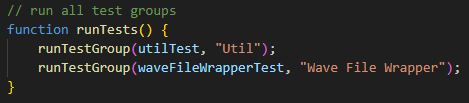
\includegraphics[width=0.8\textwidth]{../assets/add_call_to_runTestGroup.png}
    \caption{Adding a method call to run a test module}
\end{figure}

\subsubsection{Test runner}
The test runner is responsible for running the tests. It runs every test module in sequence and summarizes its results. For each module a table in the result page is created which contains the test names, result and in the case of a failed test a message why it failed. The tests are run when the dedicated button in the frontend is pressed. The test runner always runs every test of every test module. There is currently no function to run individual modules or tests.
The test runner also has a function to just test the WaveFileWrapper. It creates such a WaveFileWrapper object from the file specified on the result page and displayes the values of its properies.

\subsubsection{HTML page}
The fronted page of the test framework is used to start the tests and view the results. It is additionaly used to create a WaveFileWrapper object and view the properties of it. The test page is accessible under /js/test/test.html. To run the test page localy, see chapter 10.2.1. 

\begin{figure}[H]
    \centering
    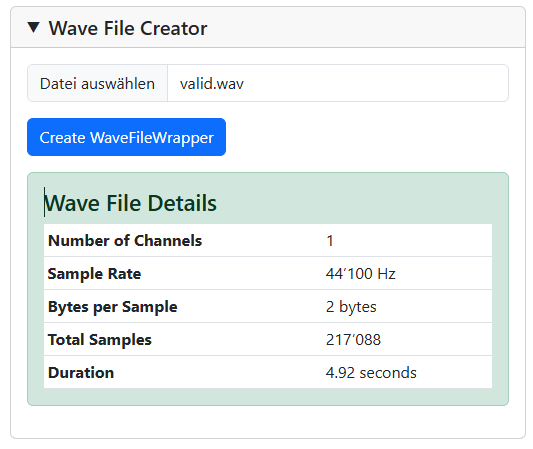
\includegraphics[width=0.8\textwidth]{../assets/wavefilecreator.png}
    \caption{Create a WaveFileWrapper object and view its properties}
\end{figure}

\begin{figure}[H]
    \centering
    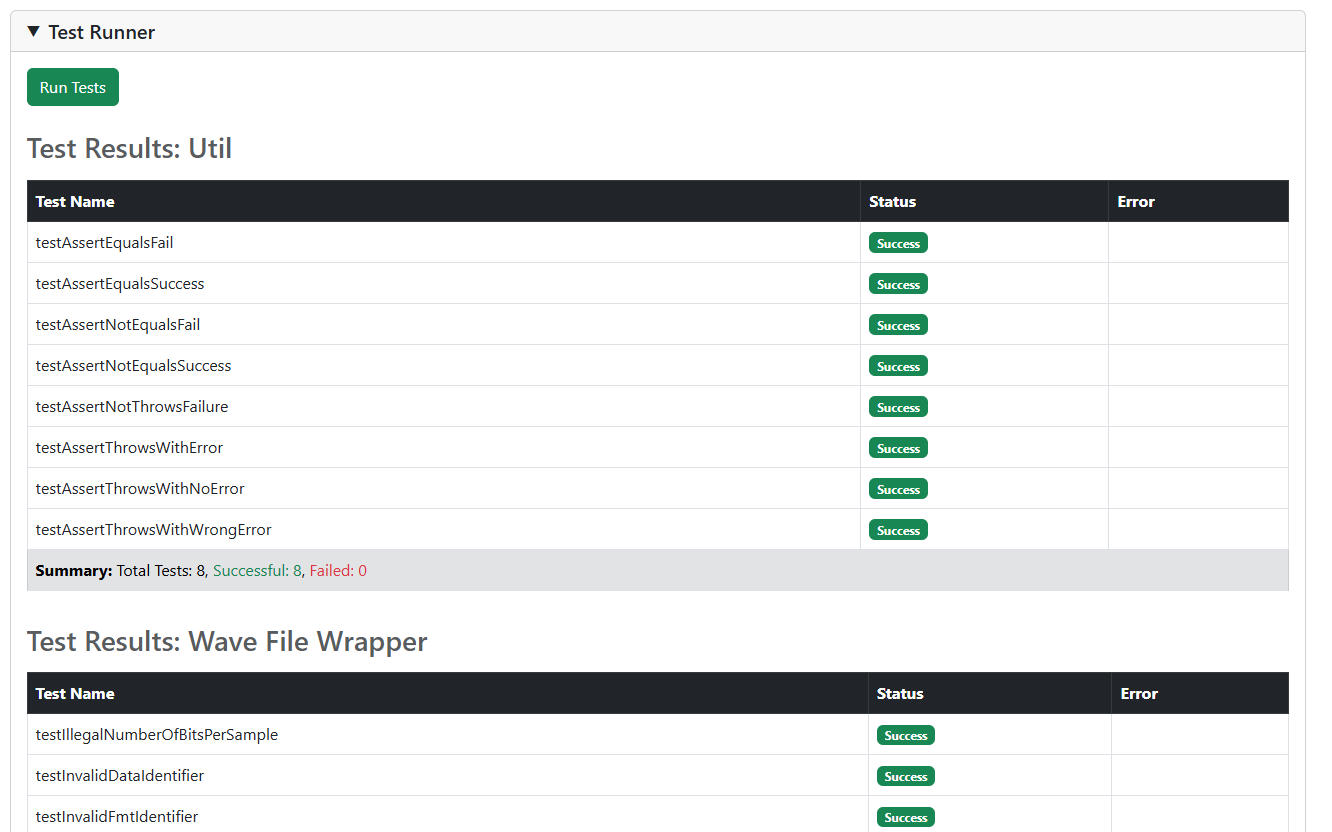
\includegraphics[width=0.8\textwidth]{../assets/test_results.png}
    \caption{Test results}
\end{figure}
